%!TEX root = ../dissertation.tex
\begin{savequote}[75mm]
Nulla facilisi. In vel sem. Morbi id urna in diam dignissim feugiat. Proin molestie tortor eu velit. Aliquam erat volutpat. Nullam ultrices, diam tempus vulputate egestas, eros pede varius leo.
\qauthor{Quoteauthor Lastname}
\end{savequote}

\chapter{Evolving (Local) Behaviors}

To evolve local behaviors, we run genetic algorithms over genomes containing
abstract syntax trees for a simple domain specific language we designed
specifically for computing a new heading from a list of neighboring agents.

\section{Domain Specific Language}
\label{sec:language}
All evolved local behaviors need to be well-defined for any number of
neighboring agents, so we choose an execution model that generalizes over the
number of neighbors a influencing agent has.
Every expression in our domain specific language defines a function from an
accumulator value representing a heading and a neighbor agent to a new
accumulator value.
Starting with an initial accumulator value, the same function is applied to
each of the influencing agent's neighbors in decreasing order of distance.
The result of each application becomes the accumulator value fed to the next
application, and the result of the final application is the heading the
influencing agent will take in the next time step.
In functional programming terms, we are evolving a function used to fold over a
list of neighbors.
The pseudocode for this fold is in listing \ref{listing:fold}.

\begin{lstlisting}[caption={A fold},captionpos=b,label={listing:fold}]
acc = initial_acc
for neighbor in neighbors:
    acc = f(acc, neighbor)
return acc
\end{lstlisting}

The order in which neighbors are evaluated is meaningful, since the evolved
functions are not necessarily commutative.
We choose to evaluate them in decreasing order of distance to ensure that the
results of programs that do not use the accumulator value are determined by the
nearest neighbor of the influencing agent.
If the influencing agent has no neighbors, its calculated heading is equal to
its initial accumulator value.
A genome is comprised of an abstract syntax tree for the folding function and
the initial accumulator value.
The initial accumulator value is either the influencing agent's current heading
or the goal direction, decided at random when an initial genome is created.
An example of a hand-crafted genome is given in listing
\ref{listing:example_genome}.

\begin{lstlisting}[caption={A small genome that sets the agent's heading to the
average of its neighbors' headings},captionpos=b,label={listing:example_genome}]
acc=current;
(add acc (mul influence heading))
\end{lstlisting}

By using a fold as our execution model, we can keep the syntax of the language
very simple.
Because the execution model handles looping over the list of neighbors, there
is no need for the language itself to have syntax expressing loops or lists.
Although allowing the language to have lists and loops would increase its
expressiveness, we opted to keep the language simple while still expressive
enough to allow the genetic algorithm to develop complex behaviors.
We also chose to leave out other possible capabilities such as mechanisms for
storing state other than the accumulator value and communicating with other
influencing agents.

The expressions that make up the domain specific language are given in table
\ref{table:lang_exprs}.
When evaluated, every expression in the language has a value in the range
$[-1,1]$, which is interpreted as an angle (in radians) by multiplying by
$\pi$.
All angles are relative to the influencing agent's current heading.
Addition, subtraction, sine, and cosine operators treat their arguments as
angles, but multiplication, exponentiation, arcsine, and arccosine treat them
as scalar values.
Division is purposefully excluded from the language because there is no
meaningful way to enforce that its result is in the range $[-1, 1]$.
Exponentiation is modified such that the exponent is implicitly shifted into
the range $[0, 2]$ to enforce the same invariant.

We determined what information should be made available about neighboring
agents by drawing on our own intuition about what information would be valuable
in designing an influencing behavior, then transforming it to be in the range
$[-1, 1]$.
For example, knowing the index of the current neighbor allows for creating a
function that gives more weight to closer neighbors (those with higher indices);
knowing the distance to the current neighbor combined with the conditional
expression, gez, allows for creating programs that ignore neighbors that are
too close or too far away;
and the product of the influence variable and some other value can be added to
the accumulator to calculate an average over all neighbors.
Figure \ref{fig:genome_diagram} shows how the direction, distance, heading, and
goal variables relate to the position of a neighboring agent.

\begin{table}[h]
\centering
\begin{tabular}{|c|c|} 
    \hline
    \textbf{Expression} & \textbf{Semantics} \\
    \hline
    direction & angle toward neighbor\\ \hline
    distance & distance to neighbor / sensing radius \\ \hline
    heading & relative heading of neighbor \\ \hline
    influence & 1 / \# of neighbors \\ \hline
    index & index of neighbor / \# of neighbors\\ \hline
    goal & angle toward goal direction \\ \hline
    acc & the accumulator value \\ \hline
    $f$ & some constant $f \in [-1, 1]$ \\ \hline
    (sin $e$) & $\sin(e\cdot\pi)$\\ \hline
    (cos $e$) & $\cos(e\cdot\pi)$\\ \hline
    (asin $e$) & $2\cdot\text{asin}(e)/\pi$\\ \hline
    (acos $e$) & $2\cdot\text{acos}(e)/\pi - 1$\\ \hline
    (add $e_1$ $e_2$) & $\text{wrap}_{[-1,1]}(e_1 + e_2)$ \\ \hline
    (sub $e_1$ $e_2$) & $\text{wrap}_{[-1,1]}(e_1 - e_2)$\\ \hline
    (mul $e_1$ $e_2$) & $e_1 \cdot e_2$\\ \hline
    (exp $e_1$ $e_2$) & $e_1^{e_2+1}$\\ \hline
    (gez $e_1$ $e_2$ $e_3$) & if $e_1 >= 0$ then $e_2$ else $e_3$ \\ \hline
\end{tabular}
\caption{Language expressions}
\label{table:lang_exprs}
\end{table}
\begin{figure}
    \centering
    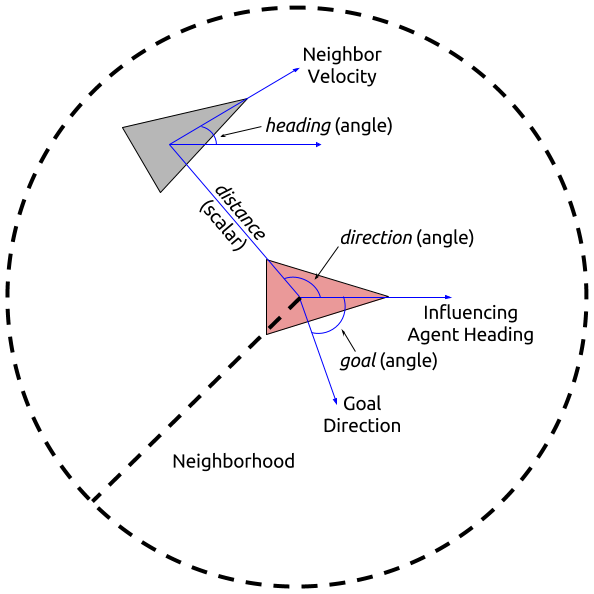
\includegraphics[width=0.4\textwidth]{genomediagram}
    \caption{Some of the variables used in the domain-specific language.}
    \label{fig:genome_diagram}
\end{figure}

To keep the language simple, angular and scalar values are used
interchangeably.
Introducing a type system to keep them separate would greatly reduce the space
of programs the genetic algorithm has to search through, at the expense of
complicating the genetic operators, which would have to respect such a type
system.
We leave implementing such a type system as well as implementing a richer
language as future work.

\section{Evolutionary Algorithm}
\label{sec:evolutionaryalg}
The two genetic operators we use in our genetic algorithm are the classic
operators in genetic programming, crossover and mutation \cite{deCastro2007}.
Crossover works by picking a random subtree from each of two abstract syntax
trees and swapping them.
Mutation picks a node at random from an abstract syntax tree and changes it
into some new node, picked uniformly at random from the set of expression types
available in the language.
The children of the old node are made children of the new node in random order,
although children may be lost if the new node has fewer children than the old
node and new children may need to be randomly generated if the new node has
more than the old node.

We start by randomly generating each member of the population.
We evaluate each member with $6$ Reynolds-Viscek agents in a small test setting,
calculating the average absolute difference in angle of the Reynolds-Viscek
agents from the goal direction after $100$ steps.
This gives a positive fitness value that we wish to optimize towards zero.
In each generation, we choose the top $N$ genomes to use as a seed population
for the next generation, where $N$ is a hyperparameter set by the user.
We add those $N$ genomes into the new population.
Then, while the size of the new population is smaller than the size of the
old population, we repeat the following:
\begin{enumerate}
    \item Flip a coin to decide whether to create a new member(s) by mutation
    or crossover.
    \item If mutation, randomly select one genome from the seed population,
    mutate it, and add it to the new population.
    \item If crossover, randomly select two genomes from the seed population,
    and use them to perform crossover.
    This creates two new offspring; add them both if there is room, otherwise
    randomly select one to add.
\end{enumerate}

We experimented with a few variations on this algorithm over the course of the
project.
We started by choosing one individual in each generation to mutate, and randomly
replaced one individual, chosen proportionally to fitness (keeping in mind that
closer to $0$ is better).
However, it was difficult for this algorithm to favor better candidates, since
fitness values were so close to each other.
We tried switching to a rank-proportional replacement algorithm, but this
approach had the opposite problem of distinguishing too finely between genomes
with very similar fitness.
We ultimately settled on our seed population approach as a compromise between
these two forces.
We also initially evolved genomes without the bias towards shorter genomes,
but we found that this let to blow-out as soon as we added crossover.
